\documentclass[letter,10pt]{article}
\usepackage[letterpaper, lmargin=.5in, rmargin=.5in]{geometry}
\usepackage[utf8]{inputenc}
\usepackage{verbatim}
\usepackage{color}
\usepackage{amsmath}
\usepackage{listings}
\usepackage{amssymb}
\usepackage{amsfonts}
\usepackage{graphicx}
\usepackage{subfig}
% \usepackage{pstool}
\usepackage{algorithm}
\usepackage{array}
\usepackage[binary-units]{siunitx}
\usepackage[backref=page,
            pageanchor=true,
            plainpages=false,
            pdfpagelabels,
            bookmarks,
            bookmarksnumbered,
            linkbordercolor={1 0.5 0.5},
            citebordercolor={0 0.5 0},
]{hyperref}

\newcommand{\eg}{\textit{e.g.},~}
\newcommand{\etc}{\textit{etc.}}
\let\eqref\undefined

\newcommand{\figref}[1]{Figure~\ref{fig:#1}}
\newcommand{\algoref}[1]{Algorithm~\ref{algo:#1}}
\newcommand{\secref}[1]{Section~\ref{sec:#1}}
\newcommand{\tabref}[1]{Table~\ref{tab:#1}}
\newcommand{\eqref}[1]{Equation~\ref{eq:#1}}
\newcommand{\figlabel}[1]{\label{fig:#1}}
\newcommand{\algolabel}[1]{\label{algo:#1}}
\newcommand{\seclabel}[1]{\label{sec:#1}}
\newcommand{\tablabel}[1]{\label{tab:#1}}
\newcommand{\eqlabel}[1]{\label{eq:#1}}


% Title Page
\title{CMPSCI 453\\HW6, Wireshark Lab 3}
\author{Tony Gao}

\begin{document}
\maketitle

%\begin{abstract}
%\end{abstract}

%\section*{Collaborators And Sources}
%List everyone you have collaborated with, or discussed the assignment with,
%along with their title, contact email addresses, and nature of collaboration.
%All sources must be acknowledged.
%\paragraph{Collaborators}
%\begin{itemize}
%  \item Person One, CS PhD student,
%    \href{mailto:personone@umass.edu}{personone@umass.edu}. Discussed math
%formatting.
%  \item Person Two, Professor,
%    \href{mailto:persontwo@umass.edu}{persontwo@umass.edu}. Discussed Maxwell's
%equations.
%\end{itemize}
%\paragraph{Sources}
%\begin{itemize}
%  \item \url{https://en.wikibooks.org/wiki/LaTeX/Mathematics}
%  \item \url{http://detexify.kirelabs.org/classify.html}
%\end{itemize}

\section{Problem 1}
\begin{enumerate}

\item Run nslookup to obtain the IP address of a Web server in Asia. What is the IP address of that server? \\
\begin{verbatim}
Tonys-MBP:CS453 rpg711$ nslookup google.com.hk
Server:		192.168.1.1
Address:	192.168.1.1#53

Non-authoritative answer:
Name:	google.com.hk
Address: 172.217.9.35
\end{verbatim} 
The type A record for google.com.hk maps it to 172.217.9.35

\item Run nslookup to determine the authoritative DNS servers for a university in
Europe.

\begin{verbatim}
Tonys-MBP:CS453 rpg711$ nslookup -type=NS www.cam.ac.uk
Server:		192.168.1.1
Address:	192.168.1.1#53

Non-authoritative answer:
www.cam.ac.uk	canonical name = cam.ac.uk.
cam.ac.uk	nameserver = dns0.cl.cam.ac.uk.
cam.ac.uk	nameserver = authdns0.csx.cam.ac.uk.
cam.ac.uk	nameserver = sns-pb.isc.org.
cam.ac.uk	nameserver = dns0.eng.cam.ac.uk.
cam.ac.uk	nameserver = ns2.ic.ac.uk.

Authoritative answers can be found from:
authdns0.csx.cam.ac.uk	internet address = 131.111.8.37
sns-pb.isc.org	internet address = 192.5.4.1
sns-pb.isc.org	has AAAA address 2001:500:2e::1
dns0.eng.cam.ac.uk	internet address = 129.169.8.8
\end{verbatim}

There are 4 type NS records for official authoritative DNS servers for Cambridge University.

\item Run nslookup so that one of the DNS servers obtained in Question 2 is queried for
the mail servers for Yahoo! mail. What is its IP address?

\begin{verbatim}
Tonys-MBP:CS453 rpg711$ nslookup -type=mx yahoo.com authdns0.csx.cam.ac.uk
Server:		authdns0.csx.cam.ac.uk
Address:	131.111.8.37#53

** server can't find yahoo.com: REFUSED
\end{verbatim}

Doing an nslookup for -type=MX for yahoo.com gives mta7.am0.yahoodns.net as one of the mail servers. A type A query reveals that mta7.am0.yahoodns.net maps to many IP addresses, one of which is 98.137.159.27.

\begin{verbatim}
Tonys-MBP:CS453 rpg711$ nslookup mta7.am0.yahoodns.net
Server:		192.168.1.1
Address:	192.168.1.1#53

Non-authoritative answer:
Name:	mta7.am0.yahoodns.net
Address: 98.137.159.27
.. truncated ..
\end{verbatim}

\end{enumerate}

\section{Problem 2}

\begin{verbatim}
    143 13.265556      192.168.1.20          192.168.1.1           DNS      79     Standard query
0x5f53 A clients6.google.com
Frame 143: 79 bytes on wire (632 bits), 79 bytes captured (632 bits) on interface 0
Ethernet II, Src: Apple_10:41:06 (80:e6:50:10:41:06), Dst: AsustekC_3f:90:60 (74:d0:2b:3f:90:60)
Internet Protocol Version 4, Src: 192.168.1.20, Dst: 192.168.1.1
User Datagram Protocol, Src Port: 45190, Dst Port: 53
Domain Name System (query)
    [Response In: 144]
    Transaction ID: 0x5f53
    Flags: 0x0100 Standard query
        0... .... .... .... = Response: Message is a query
        .000 0... .... .... = Opcode: Standard query (0)
        .... ..0. .... .... = Truncated: Message is not truncated
        .... ...1 .... .... = Recursion desired: Do query recursively
        .... .... .0.. .... = Z: reserved (0)
        .... .... ...0 .... = Non-authenticated data: Unacceptable
    Questions: 1
    Answer RRs: 0
    Authority RRs: 0
    Additional RRs: 0
    Queries
        clients6.google.com: type A, class IN
    144 13.279903      192.168.1.1           192.168.1.20          DNS      119    Standard query
response 0x5f53 A clients6.google.com CNAME clients.l.google.com A 172.217.11.46
Frame 144: 119 bytes on wire (952 bits), 119 bytes captured (952 bits) on interface 0
Ethernet II, Src: AsustekC_3f:90:60 (74:d0:2b:3f:90:60), Dst: Apple_10:41:06 (80:e6:50:10:41:06)
Internet Protocol Version 4, Src: 192.168.1.1, Dst: 192.168.1.20
User Datagram Protocol, Src Port: 53, Dst Port: 45190
Domain Name System (response)
    [Request In: 143]
    [Time: 0.014347000 seconds]
    Transaction ID: 0x5f53
    Flags: 0x8180 Standard query response, No error
        1... .... .... .... = Response: Message is a response
        .000 0... .... .... = Opcode: Standard query (0)
        .... .0.. .... .... = Authoritative: Server is not an authority for domain
        .... ..0. .... .... = Truncated: Message is not truncated
        .... ...1 .... .... = Recursion desired: Do query recursively
        .... .... 1... .... = Recursion available: Server can do recursive queries
        .... .... .0.. .... = Z: reserved (0)
        .... .... ..0. .... = Answer authenticated: Answer/authority portion was not
authenticated by the server
        .... .... ...0 .... = Non-authenticated data: Unacceptable
        .... .... .... 0000 = Reply code: No error (0)
    Questions: 1
    Answer RRs: 2
    Authority RRs: 0
    Additional RRs: 0
    Queries
        clients6.google.com: type A, class IN
    Answers
        clients6.google.com: type CNAME, class IN, cname clients.l.google.com
        clients.l.google.com: type A, class IN, addr 172.217.11.46
\end{verbatim}

\begin{enumerate}
\setcounter{enumi}{3}

\item Locate the DNS query and response messages. Are then sent over UDP or TCP?

UDP

\item What is the destination port for the DNS query message? What is the source port
of DNS response message?

\textbf{Query}: User Datagram Protocol, Src Port: 45190, Dst Port: 53 \\
\textbf{Response}: User Datagram Protocol, Src Port: 53, Dst Port: 45190

\item To what IP address is the DNS query message sent? Use ipconfig to determine the
IP address of your local DNS server. Are these two IP addresses the same?

192.168.1.1. I am on a Macbook Pro OS X 10.12 so ifconfig does not list my DNS servers. Instead, scutil must be used.

\begin{verbatim}
$ scutil --dns
DNS configuration

resolver #1
  nameserver[0] : 192.168.1.1
  if_index : 7 (en0)
  flags    : Request A records
  reach    : 0x00020002 (Reachable,Directly Reachable Address)
\end{verbatim}

\item Examine the DNS query message. What “Type” of DNS query is it? Does the
query message contain any “answers”?

\begin{verbatim}
Queries
    clients6.google.com: type A, class IN
\end{verbatim}

It contains 0 answers and 1 question,  the full query is below.

\begin{verbatim}
Domain Name System (query)
    [Response In: 144]
    Transaction ID: 0x5f53
    Flags: 0x0100 Standard query
        0... .... .... .... = Response: Message is a query
        .000 0... .... .... = Opcode: Standard query (0)
        .... ..0. .... .... = Truncated: Message is not truncated
        .... ...1 .... .... = Recursion desired: Do query recursively
        .... .... .0.. .... = Z: reserved (0)
        .... .... ...0 .... = Non-authenticated data: Unacceptable
    Questions: 1
    Answer RRs: 0
    Authority RRs: 0
    Additional RRs: 0
    Queries
        clients6.google.com: type A, class IN
\end{verbatim}

\item Examine the DNS response message. How many “answers” are provided? What
do each of these answers contain?

2 answers. A canonical name mapping for clients6.google.com and a hostname-IP mapping for clients.l.google.com

\begin{lstlisting}[breaklines]
Domain Name System (response)
    [Request In: 143]
    [Time: 0.014347000 seconds]
    Transaction ID: 0x5f53
    Flags: 0x8180 Standard query response, No error
        1... .... .... .... = Response: Message is a response
        .000 0... .... .... = Opcode: Standard query (0)
        .... .0.. .... .... = Authoritative: Server is not an authority for domain
        .... ..0. .... .... = Truncated: Message is not truncated
        .... ...1 .... .... = Recursion desired: Do query recursively
        .... .... 1... .... = Recursion available: Server can do recursive queries
        .... .... .0.. .... = Z: reserved (0)
        .... .... ..0. .... = Answer authenticated: Answer/authority portion was not authenticated by the server
        .... .... ...0 .... = Non-authenticated data: Unacceptable
        .... .... .... 0000 = Reply code: No error (0)
    Questions: 1
    Answer RRs: 2
    Authority RRs: 0
    Additional RRs: 0
    Queries
    Answers
        clients6.google.com: type CNAME, class IN, cname clients.l.google.com
        clients.l.google.com: type A, class IN, addr 172.217.11.46
\end{lstlisting}

\item Consider the subsequent TCP SYN packet sent by your host. Does the destination
IP address of the SYN packet correspond to any of the IP addresses provided in
the DNS response message?

Yes.

\begin{lstlisting}[breaklines]
Internet Protocol Version 4, Src: 192.168.1.20, Dst: 172.217.11.46
Transmission Control Protocol, Src Port: 55588, Dst Port: 80, Seq: 0, Len: 0
    Source Port: 55588
    Destination Port: 80
    [Stream index: 25]
    [TCP Segment Len: 0]
    Sequence number: 0    (relative sequence number)
    Acknowledgment number: 0
    1011 .... = Header Length: 44 bytes (11)
    Flags: 0x002 (SYN)
    Window size value: 65535
    [Calculated window size: 65535]
    Checksum: 0xb461 [unverified]
    [Checksum Status: Unverified]
    Urgent pointer: 0
    Options: (24 bytes), Maximum segment size, No-Operation (NOP), Window scale, No-Operation (NOP), No-Operation (NOP), Timestamps, SACK permitted, End of Option List (EOL)

\end{lstlisting}

\item This web page contains images. Before retrieving each image, does your host
issue new DNS queries? 

No, the image wireshark capture numbers go from 603-607. DNS queries go from 84-484, 1538-1587 so there is no overlap, implying no DNS queries are done for images. This makes sense, because the images are all local to the ietf.org hostname, which was already resolved.

\end{enumerate}

\section{Problem 3 (11-15)}

\begin{enumerate}
\item What is the destination port for the DNS query message? What is the source port
of DNS response message?

\textbf{Query}: User Datagram Protocol, Src Port: 65435, Dst Port: 53 \\
\textbf{Response}: User Datagram Protocol, Src Port: 53, Dst Port: 65435

\item To what IP address is the DNS query message sent? Is this the IP address of your
default local DNS server?

Internet Protocol Version 4, Src: 192.168.1.20, Dst: 192.168.1.1 \\
Yes, this is the IP of my default DNS.


\item Examine the DNS query message. What “Type” of DNS query is it? Does the
query message contain any “answers”?

Type A. No answers.

\begin{verbatim}
Domain Name System (query)
    [Response In: 71]
    Transaction ID: 0x1e3a
    Flags: 0x0100 Standard query
        0... .... .... .... = Response: Message is a query
        .000 0... .... .... = Opcode: Standard query (0)
        .... ..0. .... .... = Truncated: Message is not truncated
        .... ...1 .... .... = Recursion desired: Do query recursively
        .... .... .0.. .... = Z: reserved (0)
        .... .... ...0 .... = Non-authenticated data: Unacceptable
    Questions: 1
    Answer RRs: 0
    Authority RRs: 0
    Additional RRs: 0
    Queries
        mit.edu: type A, class IN

\end{verbatim}

\item Examine the DNS response message. How many “answers” are provided? What
do each of these answers contain?

1 Answer. Type A response.

\begin{verbatim}
Domain Name System (response)
    [Request In: 70]
    [Time: 0.028550000 seconds]
    Transaction ID: 0x1e3a
    Flags: 0x8180 Standard query response, No error
        1... .... .... .... = Response: Message is a response
        .000 0... .... .... = Opcode: Standard query (0)
        .... .0.. .... .... = Authoritative: Server is not an authority for domain
        .... ..0. .... .... = Truncated: Message is not truncated
        .... ...1 .... .... = Recursion desired: Do query recursively
        .... .... 1... .... = Recursion available: Server can do recursive queries
        .... .... .0.. .... = Z: reserved (0)
        .... .... ..0. .... = Answer authenticated: Answer/authority portion was not authenticated by the server
        .... .... ...0 .... = Non-authenticated data: Unacceptable
        .... .... .... 0000 = Reply code: No error (0)
    Questions: 1
    Answer RRs: 1
    Authority RRs: 0
    Additional RRs: 0
    Queries
        mit.edu: type A, class IN
    Answers
        mit.edu: type A, class IN, addr 104.88.59.205
\end{verbatim}

\item Provide a screenshot.

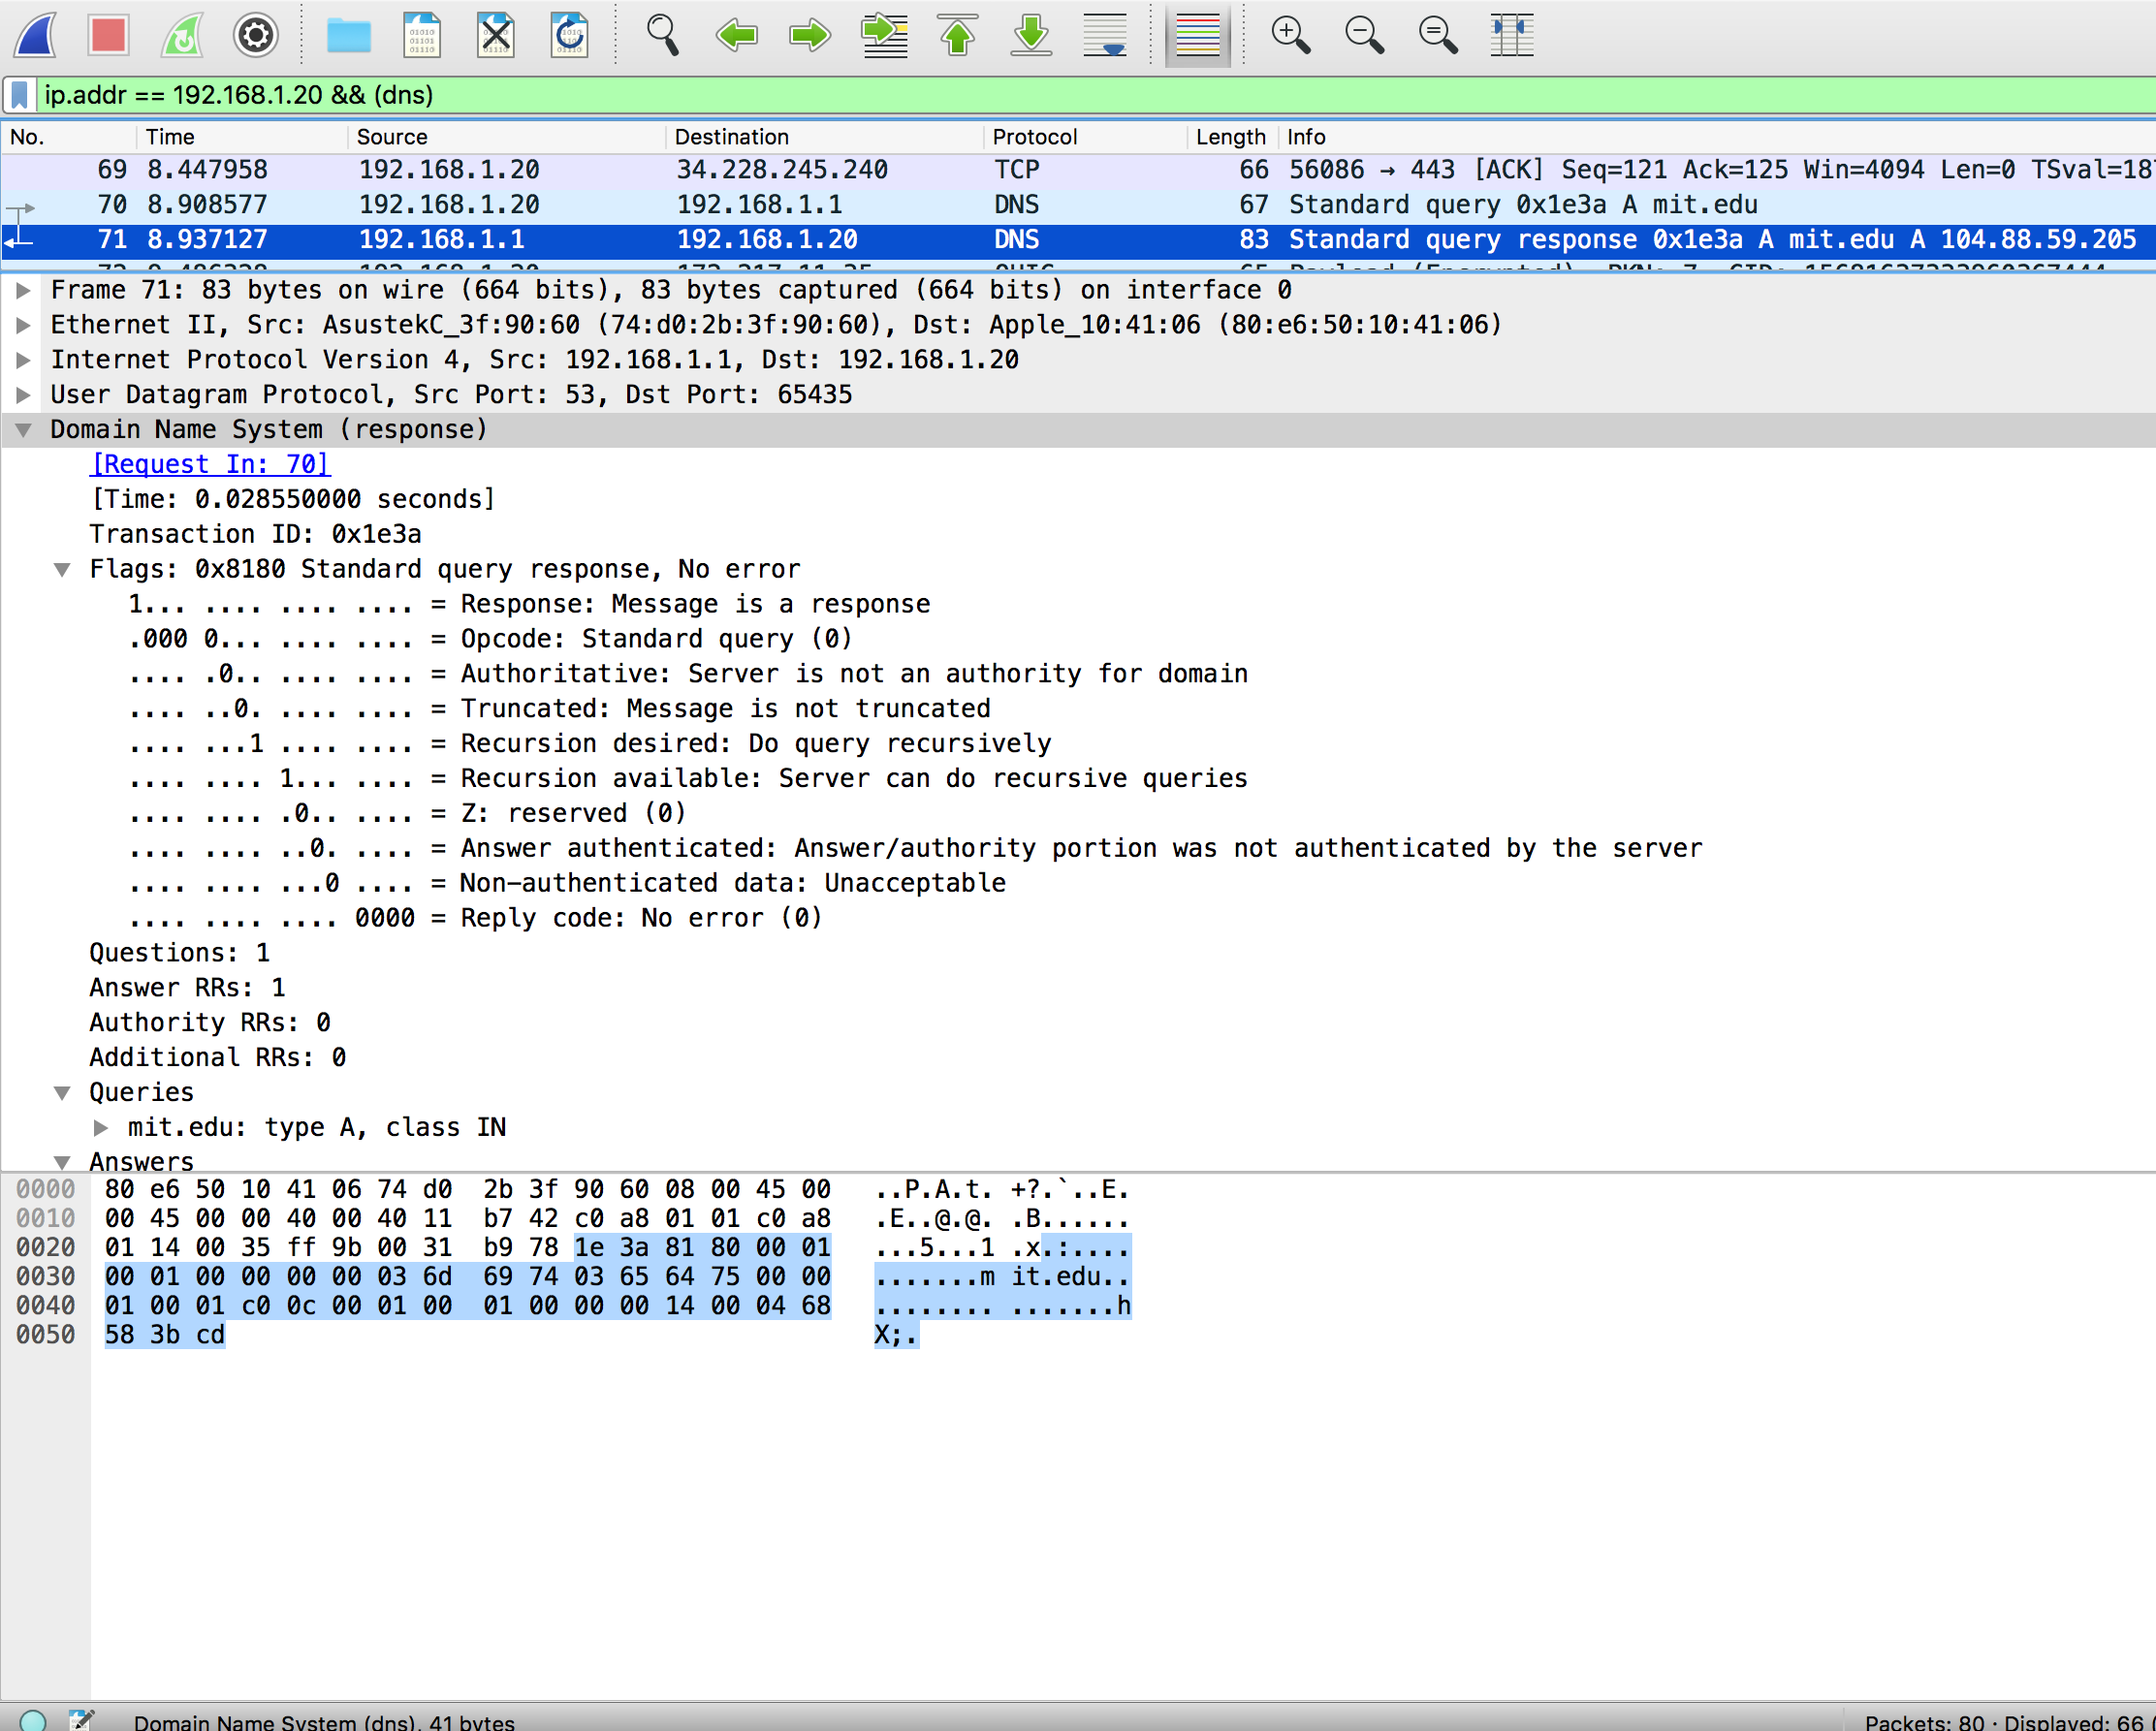
\includegraphics[width=\textwidth]{./figures/hw6_screenshot_15.png}

\end{enumerate}

\section{Problem 4 (16-19)}

\begin{enumerate}
\item To what IP address is the DNS query message sent? Is this the IP address of your
default local DNS server?

192.168.1.1. Yes

\begin{verbatim}
Internet Protocol Version 4, Src: 192.168.1.20, Dst: 192.168.1.1
\end{verbatim}

\item Examine the DNS query message. What “Type” of DNS query is it? Does the
query message contain any “answers”?

Type NS. No answers.

\begin{verbatim}
Domain Name System (query)
    [Response In: 70]
    Transaction ID: 0x3254
    Flags: 0x0100 Standard query
    Questions: 1
    Answer RRs: 0
    Authority RRs: 0
    Additional RRs: 0
    Queries
        mit.edu: type NS, class IN

\end{verbatim}

\item Examine the DNS response message. What MIT nameservers does the response
message provide? Does this response message also provide the IP addresses of the
MIT namesers?

The MIT NS are under Answers. The response does not provide IP since they are type NS responses.

\begin{verbatim}
Domain Name System (response)
    [Request In: 69]
    [Time: 0.014984000 seconds]
    Transaction ID: 0x3254
    Flags: 0x8180 Standard query response, No error
    Questions: 1
    Answer RRs: 8
    Authority RRs: 0
    Additional RRs: 9
    Queries
    Answers
        mit.edu: type NS, class IN, ns asia2.akam.net
        mit.edu: type NS, class IN, ns ns1-37.akam.net
        mit.edu: type NS, class IN, ns use5.akam.net
        mit.edu: type NS, class IN, ns use2.akam.net
        mit.edu: type NS, class IN, ns eur5.akam.net
        mit.edu: type NS, class IN, ns ns1-173.akam.net
        mit.edu: type NS, class IN, ns asia1.akam.net
        mit.edu: type NS, class IN, ns usw2.akam.net
    Additional records
        asia2.akam.net: type A, class IN, addr 95.101.36.64
        ns1-37.akam.net: type A, class IN, addr 193.108.91.37
        use5.akam.net: type A, class IN, addr 2.16.40.64
        use5.akam.net: type AAAA, class IN, addr 2600:1403:a::40
        use2.akam.net: type A, class IN, addr 96.7.49.64
        eur5.akam.net: type A, class IN, addr 23.74.25.64
        ns1-173.akam.net: type A, class IN, addr 193.108.91.173
        asia1.akam.net: type A, class IN, addr 95.100.175.64
        usw2.akam.net: type A, class IN, addr 184.26.161.64

\end{verbatim}

\item Provide a screenshot.

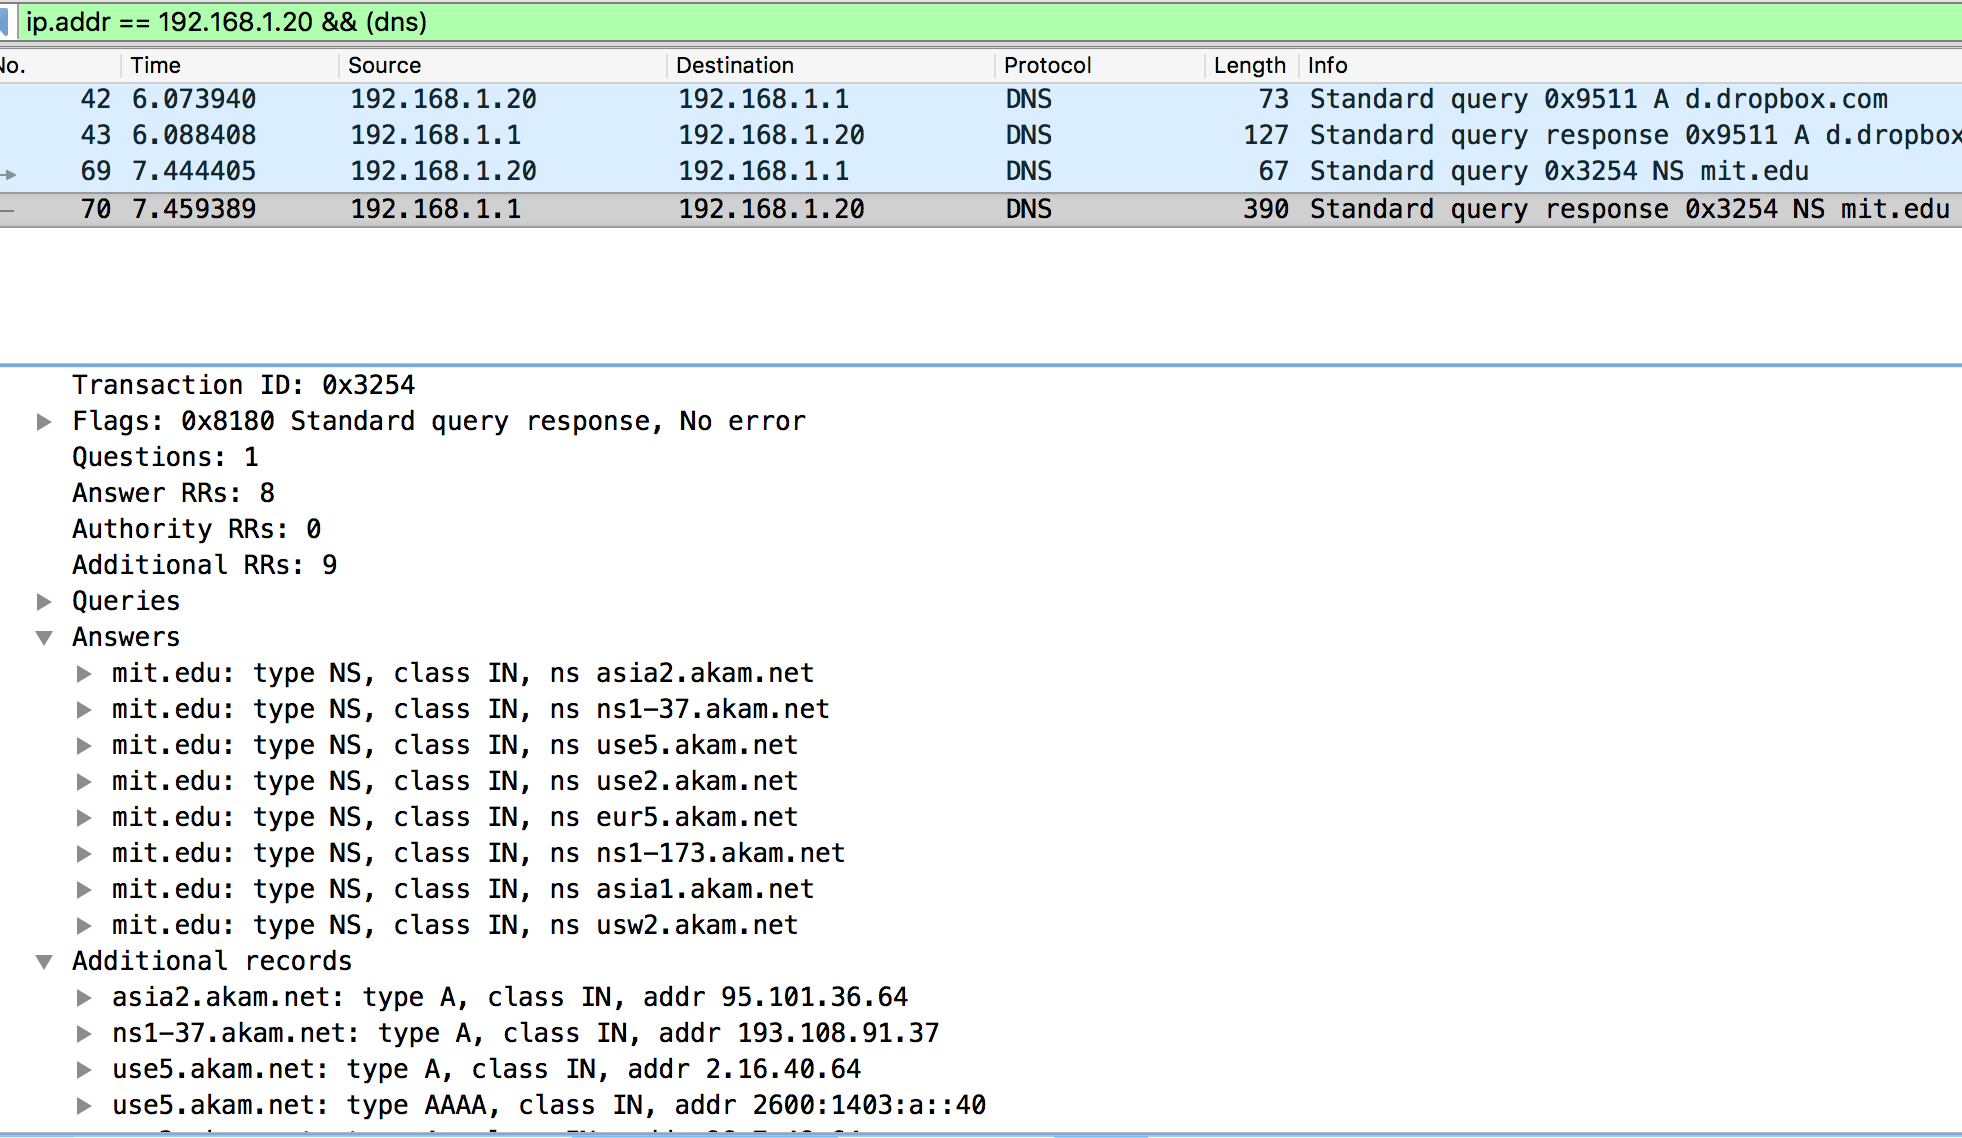
\includegraphics[width=\textwidth]{./figures/hw6_screenshot_19.png}

\end{enumerate}

\section{Problem 5(20-23)}

The given command `nslookup www.aiit.or.kr bitsy.mit.edu` contains an obsolete server. Instead I ran a nslookup of google.com against google's own DNS server (ns3.google.com).

\begin{verbatim}
$ nslookup -type=A google.com 216.239.36.10
Server:		216.239.36.10
Address:	216.239.36.10#53

Name:	google.com
Address: 172.217.12.206
\end{verbatim}

\begin{enumerate}

\item To what IP address is the DNS query message sent? Is this the IP address of your
default local DNS server? If not, what does the IP address correspond to?

Sent to 216.239.36.10. Not the IP of my local DNS server. IP corresponds to the ip address of google's dns server ns3.google.com.

\begin{verbatim}
Internet Protocol Version 4, Src: 192.168.1.20, Dst: 216.239.36.10
\end{verbatim}

\item Examine the DNS query message. What “Type” of DNS query is it? Does the
query message contain any “answers”?

Type A, no answers.

\begin{verbatim}
Domain Name System (query)
    [Response In: 99]
    Transaction ID: 0xc01c
    Flags: 0x0100 Standard query
    Questions: 1
    Answer RRs: 0
    Authority RRs: 0
    Additional RRs: 0
    Queries
\end{verbatim}

\item Examine the DNS response message. How many “answers” are provided? What
does each of these answers contain?

1 answer. Type A record for google.com

\begin{verbatim}
Domain Name System (response)
    [Request In: 98]
    [Time: 0.034990000 seconds]
    Transaction ID: 0xc01c
    Flags: 0x8500 Standard query response, No error
    Questions: 1
    Answer RRs: 1
    Authority RRs: 0
    Additional RRs: 0
    Queries
    Answers
        google.com: type A, class IN, addr 172.217.12.206

\end{verbatim}

\item Provide a screenshot.

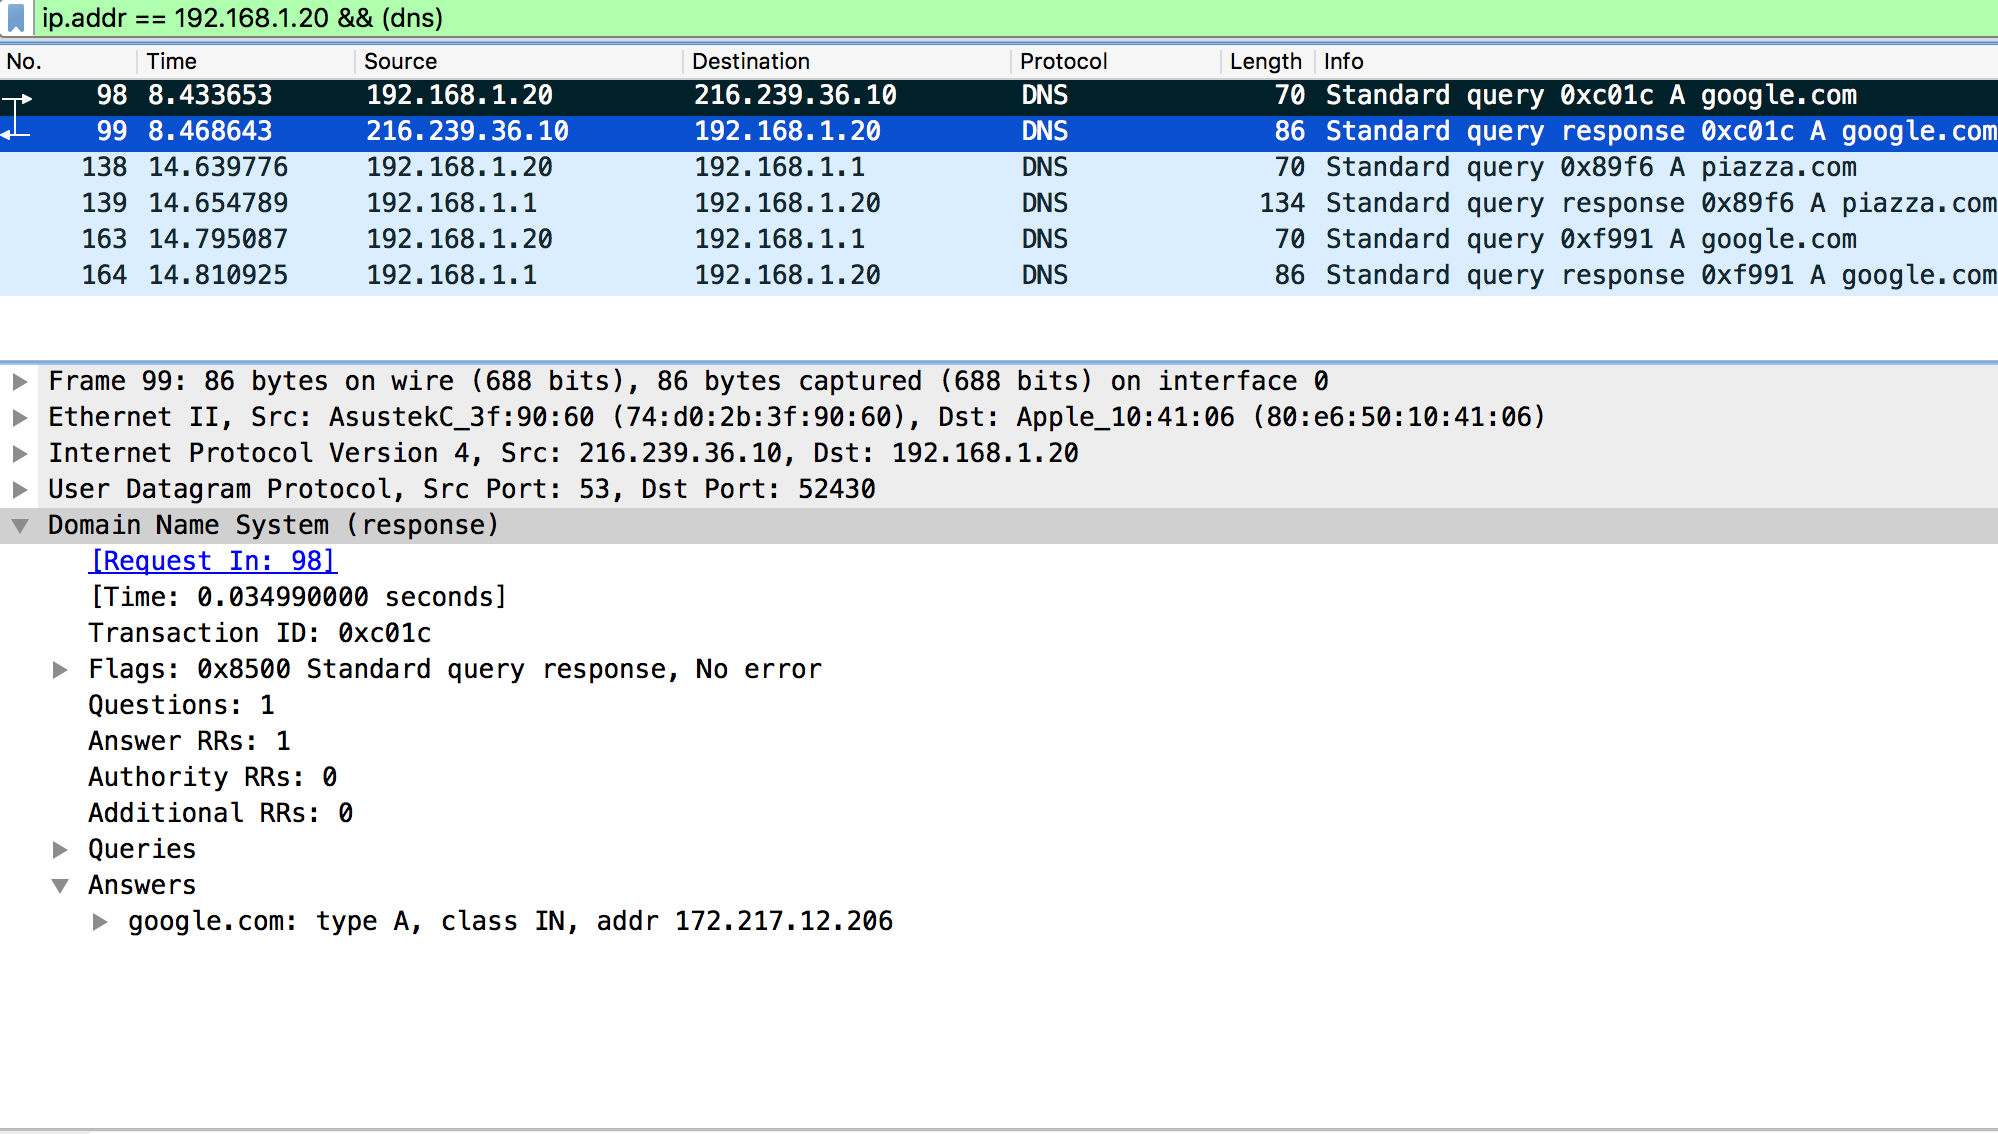
\includegraphics[width=\textwidth]{./figures/hw6_screenshot_23.png}

\end{enumerate}

\end{document}
